\section{Actividad No 09 – SubConsultas} 
		
\begin{enumerate}[1.]
	\item El departamento de Recursos Humanos requiere una consulta que pregunte al usuario por el Apellido del empleado, Luego la consulta deber\'a mostrar los Apellidos y Fecha de Contrataci\'on de todos los empleados del mismo departamento excluyendo o con excepción del empleado el cual ha sido proporcionado su apellido reporte que muestre las direcciones de todos los departamentos.
	\\
	\\-- leyendo id de empleado\\
	SET @empid \= 110\\
	-- obteniendo id de departamento de empleado \\
	SET @depid \= (SELECT emp.department\_id \\
	FROM employees as emp \\
	WHERE emp.employee\_id\=@empid); \\
	-- todos los empleados del mismo departamento excluyendo al empleado ingresado anteriormente\\
	SELECT emp.employee\_id, \\
	emp.last\_name, \\
	emp.hire\_date, \\
	emp.department\_id \\
	FROM employees AS emp \\
	WHERE emp.department\_id\=@depid \\
	AND emp.employee\_id!\=@empid; \\
	\begin{center}
	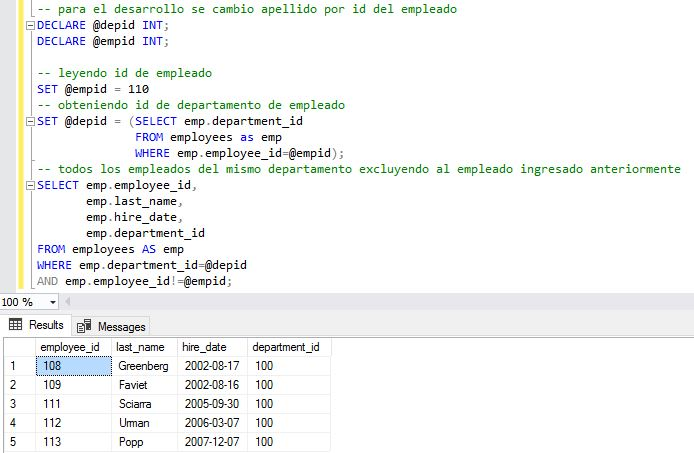
\includegraphics[width=5cm]{./Imagenes/actividad0901} 
	\end{center}

	\item Crear un reporte que muestre el No del Empleado, Apellidos y Salarios de todos los empleados que tienen un salario superior al promedio de salarios de todos los empleados. Ordenar los resultados por el Salario de forma ascendente.
	\\
	\\SELECT emp.employee\_id, \\
	emp.last\_name, \\
	emp.salary \\
	FROM employees AS emp \\
	WHERE emp.salary>@prom; \\
	\begin{center}
	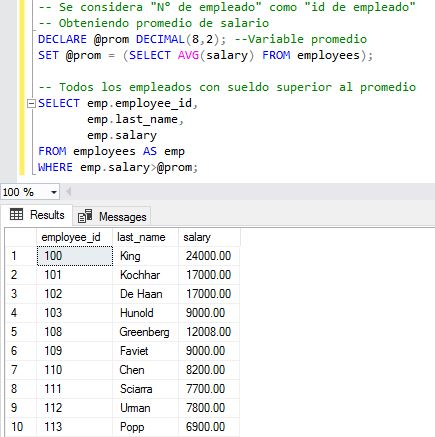
\includegraphics[width=5cm]{./Imagenes/actividad0902} 
	\end{center}

	\item Realizar un reporte que muestre el No de Empleado y Apellidos de todos los empleados quienes trabajan en el departamento de cualquier empleado que su apellido contenga la letra ‘u’.
	\\
	\\SELECT emp.employee\_id, \\
	emp.last\_name, \\
	emp.department\_id \\
	FROM employees AS emp \\
	JOIN (SELECT DISTINCT department\_id \\
		  FROM employees \\
		  WHERE last\_name LIKE '\%u\%') AS depid \\
	ON emp.department\_id\=depid.department\_id; \\
	\begin{center}
	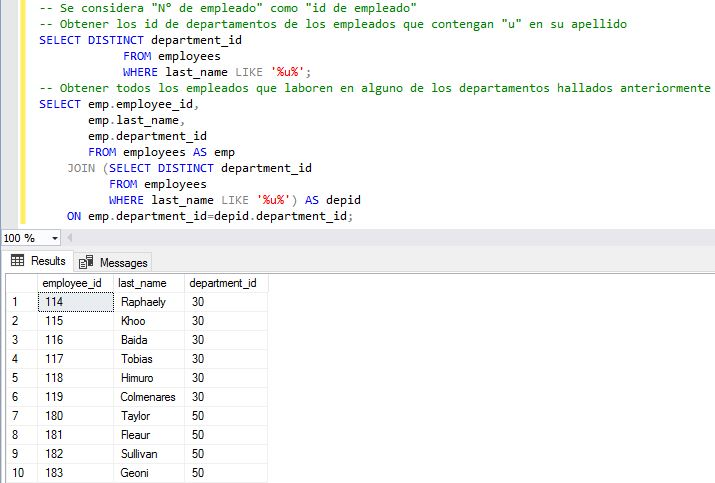
\includegraphics[width=5cm]{./Imagenes/actividad0903} 
	\end{center}

	\item El departamento de Recursos Humanos requiere un reporte que muestre los Apellidos, No de Departamento y Puestos de los empleados cuya locación de departamento es 1700.
	\\
	\\SELECT emp.last\_name, \\
	emp.department\_id, \\
	dep.location\_id \\
	FROM employees as emp \\
	JOIN departments as dep \\
	ON emp.department\_id\=dep.department\_id \\
	WHERE dep.location\_id\=1700;\\
	\begin{center}
	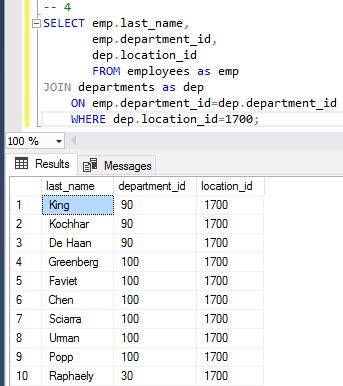
\includegraphics[width=5cm]{./Imagenes/actividad0904} 
	\end{center}

	\item Modificar la consulta anterior de forma que el usuario pueda introducir el No de locaci\'on.
	\\
	\\DECLARE @locid INT; \\
	SET @locid \= 1700; \\
	SELECT emp.last\_name, \\
	   emp.department\_id, \\
	   dep.location\_id \\
	   FROM employees as emp \\
	JOIN departments as dep \\
	ON emp.department\_id\=dep.department\_id \\
	WHERE dep.location\_id\=@locid; \\
	\begin{center}
	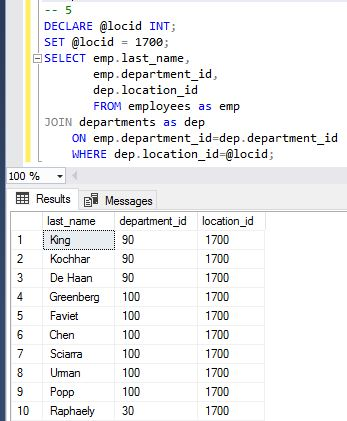
\includegraphics[width=5cm]{./Imagenes/actividad0905} 
	\end{center}

	\item Crear un reporte para el departamento de Recursos Humanos que muestre los Apellidos y Salarios de todos los empleados cuyo Administrador apellide ‘King’.
	\\
	\\SELECT emp.last\_name, \\
	   emp.salary \\
	   FROM employees AS emp \\
	JOIN (SELECT dep.department\_id \\
			 FROM departments AS dep \\
	  JOIN (SELECT employee\_id, \\
			       last\_name \\
				   FROM employees \\
				   WHERE last\_name\='KING') AS manking \\
	  ON dep.manager\_id\=manking.employee\_id) AS depking \\
	ON emp.department\_id\=depking.department\_id; \\
	\begin{center}
	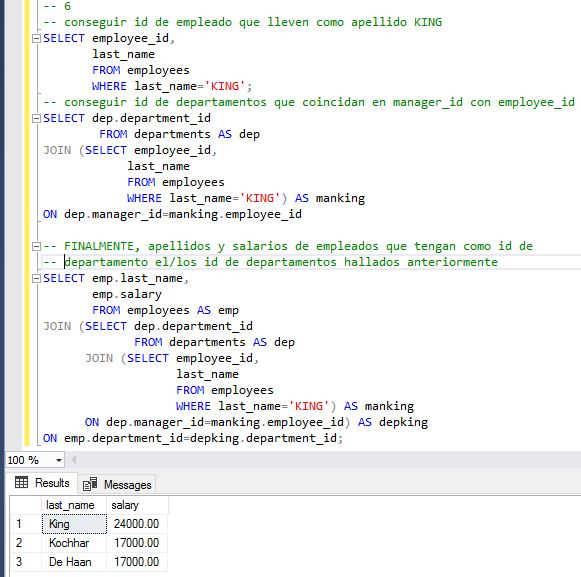
\includegraphics[width=5cm]{./Imagenes/actividad0906} 
	\end{center}

	\item Crear un reporte para el departamento de Recursos Humanos que muestre el No de Departamento, Apellidos, Puestos de todos los empleados en el departamento ‘Executive’.
	\\
	\\SELECT empnomjob.department\_id, \\
	   empnomjob.last\_name, \\
	   empnomjob.job\_title \\
	   FROM departments \\
	JOIN (SELECT emp.department\_id, \\
			 emp.last\_name, \\
			 jobs.job\_title \\
			 FROM employees AS emp \\
	  JOIN jobs \\
	  ON emp.job\_id\=jobs.job\_id) AS empnomjob \\
	ON empnomjob.department\_id\=departments.department\_id \\
	WHERE department\_name\='executive' \\

	\begin{center}
	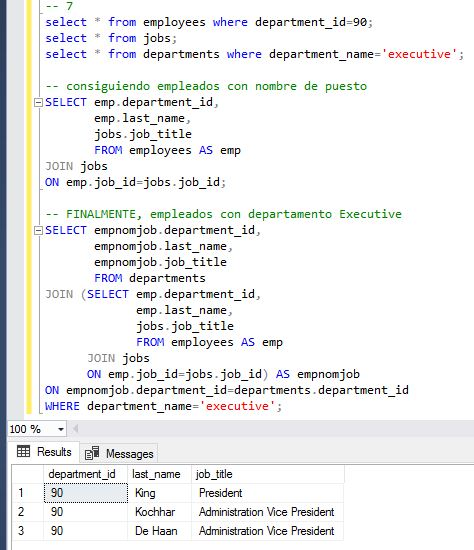
\includegraphics[width=5cm]{./Imagenes/actividad0907} 
	\end{center}

	\item Modificar la consulta del ítem 4.3 para que adicionalmente se muestro solo a los empleados que tengan un salario mayor al promedio de todos los salarios de los empleados.



\end{enumerate}
